\documentclass{article}
\usepackage{graphicx} 
\usepackage{multirow}
\usepackage{enumitem}
\usepackage{amssymb}
\usepackage{amsmath}
\usepackage{xcolor}
\usepackage{cancel}
\usepackage{tcolorbox}
\usepackage{physics}
\usepackage{geometry}
\usepackage{tikz}
\usepackage{tikz-3dplot}
\usepackage{pgfplots, tkz-euclide,calc}
    \usetikzlibrary{patterns,snakes,shapes.arrows,3d}
    \usepgfplotslibrary{fillbetween}
	\geometry{
		total = {160mm, 237mm},
		left = 25mm,
		right = 35mm,
		top = 30mm,
		bottom = 30mm,
	}

\newcommand{\jawab}{\textbf{Jawab}:}
\newcommand{\del}{\partial}
\begin{document}
    \pagenumbering{gobble}
    \begin{tabular}{|lcl|}
     \hline
     Nama&:&Teosofi Hidayah Agung\\
     NRP&:&5002221132\\
     \hline
    \end{tabular}
    \begin{enumerate}
        \item Diberikan $F=2xy^2\hat{i}+xyz\hat{j}+yz^2\hat{k}$
        \begin{enumerate}
            \item $\curl F$ di titik $P(0,1,2)$\\
            \jawab
            \begin{flalign*}
                \curl F &= \begin{vmatrix}
                    \hat{i} & \hat{j} & \hat{k}\\
                    \del_x & \del_y & \del_z\\
                    2xy^2 & xyz & yz^2
                \end{vmatrix}&\\
                &= \left(\del_y(yz^2)-\del_z(xyz)\right)\hat{i}-\left(\del_x(yz^2)-\del_z(2xy^2)\right)\hat{j}+\left(\del_x(xyz)-\del_y(2xy^2)\right)\hat{k}&\\
                &= (z^2-xy)\hat{i} + (yz-4xz)\hat{k}&\\
                \curl F_{(0,1,2)} &= (4-0)\hat{i} + (2-0)\hat{k} = 4\hat{i}+2\hat{k}
            \end{flalign*}
            \item $\curl (\curl F)$ di titik $P(0,1,2)$\\
            \jawab
            \begin{flalign*}
                \curl(\curl F) &= \begin{vmatrix}
                    \hat{i} & \hat{j} & \hat{k}\\
                    \del_x & \del_y & \del_z\\
                    z^2-xy & 0 & yz-4xz
                \end{vmatrix}&\\
                &= \del_y(yz-4xz)\hat{i}-\left(\del_x(yz-4xz)-\del_z(z^2-xy)\right)\hat{j}+(-\del_{y}(z^2-xy))\hat{k}&\\
                &= z\hat{i}-\left(-4z-2z\right)\hat{j}-(-x)\hat{k}&\\
                &= z\hat{i}+6z\hat{j}+x\hat{k}&\\
                \curl(\curl F)_{(0,1,2)} &= 2\hat{i}+12\hat{j}
            \end{flalign*}
        \end{enumerate}
        \item Hitung $\displaystyle \int_C F\cdot dr$ dimana $F=3x^2y\hat{i}-y\sqrt{x}\hat{j}$ dan $C$ adalah Lintasan yang melalui garis lurus dari $(1,0)$ ke $(2,1)$, kemudian garis lurus dari $(2,1)$ ke $(0,2)$, dan kemudian parabola $y=2-x^2$ dari $(0,2)$ ke $(-\sqrt{2},0)$. Gambarkan juga lintasan $C$ nya\\
        \jawab\\
        Lintasan $C$ dapat digambarkan sebagai berikut
        \begin{center}
            \begin{tikzpicture}
                \draw[->] (-2,0) -- (3,0) node[right] {$x$};
                \draw[->] (0,-1) -- (0,3) node[above] {$y$};
                \draw[blue] (1,0) node[below] {\footnotesize$(1,0)$} -- (2,1) node[right] {\footnotesize$(2,1)$} -- (0,2) node[above] {\footnotesize$(0,2)$};
                \draw[blue,domain=0:-{sqrt(2)},smooth] plot (\x, {2-\x*\x}) node[below] {\footnotesize$(-\sqrt{2},0)$};
            \end{tikzpicture}
        \end{center}
        Kita pecah lintasan $C$ menjadi 3 bagian, yaitu garis lurus dari $(1,0)$ ke $(2,1)$, garis lurus dari $(2,1)$ ke $(0,2)$, dan parabola $y=2-x^2$ dari $(0,2)$ ke $(-\sqrt{2},0)$.\\
        \begin{itemize}
            \item $C_1$ adalah garis lurus dari $(1,0)$ ke $(2,1)$ dengan persamaan parametrik $x=t$ dan $y=t-1$ untuk $1\leq t\leq 2$.
            \begin{flalign*}
                \int_{C_1} F\cdot dr &= \int_{1}^{2} F\cdot dr = \int_{1}^{2} (3t^2(t-1)\hat{i}-(t-1)\sqrt{t}\hat{j})\cdot (dt\hat{i}+dt\hat{j})&\\
                &= \int_{1}^{2} 3t^3(t-1)-(t-1)\sqrt{t}\,dt&\\
                &= \int_{1}^{2} 3t^4-3t^3-t\sqrt{t}+\sqrt{t}\,dt&\\
                &= \left[\frac{3}{5}t^5-\frac{3}{4}t^4-\frac{2}{5}t^{\frac{5}{2}}+\frac{2}{3}t^{\frac{3}{2}}\right]_{1}^{2}&\\
                &= \frac{3}{5}(32)-\frac{3}{4}(16)-\frac{2}{5}(4\sqrt{2})+\frac{2}{3}(2\sqrt{2})-\left(\frac{3}{5}-\frac{3}{4}-\frac{2}{5}+\frac{2}{3}\right)&\\
                &= \frac{96}{5}-12-\frac{8}{5}\sqrt{2}+\frac{4}{3}\sqrt{2}-\frac{3}{5}+\frac{3}{4}+\frac{2}{5}-\frac{2}{3}&\\
                &= \frac{425-16\sqrt{2}}{60}
            \end{flalign*}
            \item $C_2$ adalah garis lurus dari $(2,1)$ ke $(0,2)$ dengan persamaan parametrik $x=2-t$ dan $y=1+t$ untuk $0\leq t\leq 2$.
            \begin{flalign*}
                \int_{C_2} F\cdot dr &= \int_{0}^{2} F\cdot dr = \int_{0}^{2} (3(2-t)^2(1+t)\hat{i}-(1+t)\sqrt{2-t}\hat{j})\cdot (-dt\hat{i}+dt\hat{j})&\\
                &= \int_{0}^{2} 3(2-t)^2(1+t)+(1+t)\sqrt{2-t}\,dt&\\
                &= \int_{0}^{2} 3(4-4t+t^2)(1+t)+(1+t)\sqrt{2-t}\,dt&\\
                &= \int_{0}^{2} 3(4-4t+t^2+4t-4t^2+t^3)+(1+t)\sqrt{2-t}\,dt&\\
                &= \int_{0}^{2} 12t-3t^2+3t^3+(1+t)\sqrt{2-t}\,dt&\\
                &= \left[6t^2-t^3+\frac{3}{4}t^4-2(2-x)\sqrt{2-x}+\frac{2\sqrt{2-x}}{5}(4-4x+x^2)\right]_{0}^{2}&\\
                &= 12+\frac{12\sqrt{2}}{5}
            \end{flalign*}
            \item $C_3$ adalah parabola $y=2-x^2$ dari $(0,2)$ ke $(-\sqrt{2},0)$ dengan persamaan parametrik $x=-t$ dan $y=2-t^2$ untuk $0\leq t\leq \sqrt{2}$.
            \begin{flalign*}
                \int_{C_3} F\cdot dr &= \int_{0}^{\sqrt{2}} F\cdot dr = \int_{0}^{\sqrt{2}} (3(-t)^2(2-t^2)\hat{i}-(2-t^2)\sqrt{-t}\hat{j})\cdot (-dt\hat{i}-2t\,dt\hat{j})&\\
                &= \int_{0}^{\sqrt{2}} 3t^2(2-t^2)-2t(2-t^2)\sqrt{t}\,dt&\\
                &= \int_{0}^{\sqrt{2}} 6t^2-3t^4-4t\sqrt{t}+2t^3\sqrt{t}\,dt&\\
                &= \left[2t^3-t^5-\frac{8}{5}t^{\frac{5}{2}}+\frac{4}{3}t^{\frac{7}{2}}\right]_{0}^{\sqrt{2}}&\\
                &= \frac{8\sqrt{2}}{5}+\frac{16\sqrt[4]{8}}{21}
            \end{flalign*}
        \end{itemize}
        Sehingga, $\displaystyle \int_C F\cdot dr = \int_{C_1} F\cdot dr + \int_{C_2} F\cdot dr + \int_{C_3} F\cdot dr = \frac{425+4\sqrt{2}}{60}+12+\frac{16\sqrt[4]{8}}{21}$.

        \item Dengan Teorema Green, hitung $\displaystyle \int_C F\cdot dr$ dimana $F=(x^2y+3y^2)\hat{i}+(x-y^3)\hat{j}$ dan $C$ adalah lintasan yang melalui garis lurus dari $(0,0)$ ke $(1,2)$, kemudian garis lurus dari $(1,2)$ ke $(0,2)$, dan selanjutnya melewati parabola $x=y^2-2y$ dari $(0,2)$ ke $(0,0)$.\\
        \jawab\\
        Lintasan $C$ dapat digambarkan sebagai berikut
        \begin{center}
            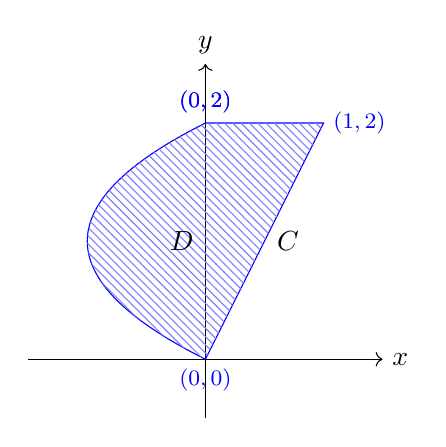
\begin{tikzpicture}[scale=1.5]
                \draw[->] (-1.5,0) -- (1.5,0) node[right] {$x$};
                \draw[->] (0,-0.5) -- (0,2.5) node[above] {$y$};
                \draw[blue,smooth, name path=A] (0,0) node[below] {\footnotesize$(0,0)$} -- (1,2) node[right] {\footnotesize$(1,2)$} -- (0,2) node[above] {\footnotesize$(0,2)$};
                \draw[blue,domain=0:2,smooth,name path=B] plot ({\x*\x-2*\x}, {\x}) node[above] {\footnotesize$(0,2)$};
                \fill [pattern=north west lines, pattern color=blue!50,domain=0:2] (0,0) -- (1,2) -- (0,2) -- plot ({\x*\x-2*\x}, {\x});

                \node[] at (0.7,1) {$C$};
                \node[] at (-0.2,1) {$D$};
            \end{tikzpicture}
        \end{center}
        Dengan menggunakan Teorema Green, kita dapat menghitung 
        \[\displaystyle \int_C M\,dx+N\,dy = \iint_D \left(\frac{\del N}{\del x}-\frac{\del M}{\del y}\right)\,dA\] 
        dimana $D$ adalah daerah yang dibatasi oleh lintasan $C$.\\
        \begin{flalign*}
            \int_C (x^2y+3y^2)\,dx+(x-y^3)\,dy &= \iint_D \left(\frac{\del(x-y^3)}{\del x}-\frac{\del(x^2y+3y^2)}{\del y}\right)\,dA&\\
            &= \iint_D (1-x^2-6y)\,dA&\\
            &= \int_{0}^{2}\int_{y^2-2y}^{y/2} (1-x^2-6y)\,dx\,dy&\\
            &= \int_{0}^{2} \left[x-\frac{1}{3}x^3-6xy\right]_{y^2-2y}^{y/2}\,dy&\\
            &= \int_{0}^{2} \left[\frac{y}{2}-\frac{y^3}{24}-3y^2-(y^2-2y)+\frac{1}{3}(y^2-2y)+6(y^2-2y)y\right]\,dy&\\
            &= \int_{0}^{2} \frac{143}{24}y^3-\frac{47}{3}y^2+\frac{11}{6}y\,dy&\\
            &= \left[\frac{143}{96}y^4-\frac{47}{9}y^3+\frac{11}{12}y^2\right]_{0}^{2}&\\
            &= -\frac{257}{18}
        \end{flalign*}
    \end{enumerate}
\end{document}